\chapter{Digital Filters}

The signals from the encoders and sensors contain uncertainties and noise, which are disturbances in the system. One way to minimize the disturbances is to implement filters which attenuate the noise and measurement uncertainties. Generally, there are two types of filters that can be implemented either analog or digital filters. Analog filters work in continuous time and digital filters in discrete time. Where the continuous time filter has a particular value of a signal at any given time, the discrete time only has defined values at specific points in time. These points are called samples and the time interval between each sample is the sampling period $T_s$ with a sampling frequency $f_s = \frac{1}{T_s}$. Since the hardware platform of the segway is provided, it might be inconvenient to extend the platform with additional hardware, i.e. if a high order filter is needed, more components are needed to realize the filter. Another issue is to design and implement analog filters, as it is not as flexible as a digital filter, since changing the filter characteristic requires changing components. A disadvantage of digital filters is the demand of computational power to realize the filters. However since a digital filters are more flexible to work with, digital filters are chosen to be implemented. Two digital filters will be designed and three implemented, since the segway has two encoders and one angle measurement. The chapter is divided into the following sections:
\begin{itemize}
\item \textbf{Spectrum analysis}\\
This section analyse the measurements from the encoders and the angle derived from the gyroscope and accelerometer sensors. The encoders for both wheels are used for measuring the speed while the gyroscope and accelerometer sensors are used to obtain the angle.
\item \textbf{Requirements and specifications for the digital filters}\\
From the spectrum analysis it is possible to set up requirements and specifications for the digital filters.
\item \textbf{Designing the digital filters}\\
The requirements and specification are in this section used to design the digital filters.
\item \textbf{Implementation of the digital filters}\\
The digital filters from previous section are implemented in the microcontroller in this section.
\end{itemize}
The first part of this chapter is the spectrum analysis, where the requirements and specifications are derived.
\section{Spectrum Analysis}
Before designing the filters, the requirements for the digital filters need to be specified. It is decided that digital filters will be implemented on both the encoders and the sensors for the angle. Requirements and specifications will be based on a spectrum analysis of the measurements from the encoders and these sensors. In this chapter the sensors used for calculating the angle, will be referred to as "sensors". The first analysis is based on the measurements from the sensors measured with the controller from a previous section implemented. The sampling period $T_s$ is set to 15 ms and the output plotted in \autoref{fig:input_gyro} is the angle derived from the sensors.

%\begin{figure}[H]
%    \centering
%    \includegraphics[width = 0.95\textwidth]{filters/input_gyro2.png}
%    \caption{Angle measurements. The measurements are taken while the segway stabilises itself in an upright position with the controller from previous section implemented.}
%    \label{fig:input_gyro}
%\end{figure} 

\begin{figure}[H]
\centering
\begin{subfigure}[b]{0.95\textwidth}
\hspace*{-0.6cm} 
    \includegraphics[width = 1\textwidth]{filters/input_gyro2.png}
    \caption{Angle measurements. The measurements are taken while the segway stabilises itself in an upright position with the controller from previous section implemented.}
    \label{fig:input_gyro}
\end{subfigure}    
\begin{subfigure}[b]{0.98\textwidth}
    \includegraphics[width = 1\textwidth]{filters/spectrogram_gyro3.png}
    \caption{Spectrogram of the angle measurements. The sampling frequency $f_s$ for both the gyroscope and the accelerometer is 66.67 Hz, window size is 20 samples and overlapping is 19 samples.}
    \label{fig:spectrogram_gyro}
\end{subfigure}   
\caption{Measured angle and spectrogram of the measured angle.}
\end{figure}

\autoref{fig:input_gyro} shows the angle when the segway, from upright position, is stabilising itself. Error measurements occur when the angle suddenly increases or decreases, see \autoref{fig:input_gyro} at 2.4 seconds, and attenuating these errors are desirable. From the angle measurements, it is seen that the segway moves forward and backwards with a period on approximately two seconds. After seven seconds the segway quickly moves forward and backwards, because a disturbance might have caused it to overreact. Designing a filter to the angle measurements, the attenuation must not be too high at frequencies where the segway overreacts, which for instance occurs at about 7 seconds in the angle measurements. Another side effect is the measurements being delayed, which is not desirable in a control system. Therefore the specifications for the filters need to be set carefully. To determine the specifications for the passband and stopband frequencies, a spectrum analysis is needed.

The measurements from \autoref{fig:input_gyro} are now spectrum analysed in the spectrogram, see \autoref{fig:spectrogram_gyro}. The spectrogram is generated from a MATLAB function which calculates multiple Discrete Fourier Transformations (DFT) of a signal. The spectrogram shows the spectrum analysis of the measurements. Because the measurements are time discrete the DFT is used instead of the Continuous Fourier Transformation (CFT). The spectrogram consists of multiple processed DFTs. The number of DFTs is determined by the window size of each DFT and the overlapping for each DFT. The window size is the length of the signal that is processed and the overlap is how much of the signal from the previous DFT is included in the next DFT. The window size is set to 20 samples, the overlap to 19 to increase the resolution of the spectogram. 	The sampling frequency of the measurements is 66.67 Hz.

%\begin{figure}[H]
%    \centering
%    \includegraphics[width = 0.9\textwidth]{filters/spectrogram_gyro3.png}
%    \caption{Spectrogram of the angular velocity. The sampling frequency $f_s$ for both the gyroscope and the accelerometer is 200 Hz, window size is 20 samples, and overlapping is 19 samples.}
%    \label{fig:spectrogram_gyro}
%\end{figure} 
A low-pass filter can be implemented to attenuate noise above 15 Hz. This is derived from comparing the amplitude plot of the measurements with the spectrogram between the 7th and 8th second. It is approximated that most of the valid measurements are between 0 to 15 Hz. To remove noise and measurement errors the cutoff frequency is set to 15 Hz.

\subsection{Spectrum Analysis for Encoders}
The specifications of the digital filter for the encoders are derived from a spectrum analysis of measurements as well with the controller implemented. However the measurements are made independently from the previous measurement for the angle sensors. The measurements are made with a sampling frequency, $f_s$, of 1 kHz and are seen in \autoref{fig:input_encoder}. The speed of the motors is in- and decreasing with a period of approximately 1 Hz, which suggests that the segway is moving forward and backwards to stabilise itself. Since it is not desirable to attenuate valid measurements, the attenuation at the passband frequency $\Omega_p$ is set to maximum 1 dB at 5 Hz.
\begin{figure}[H]
\centering
\begin{subfigure}[b]{0.95\textwidth}
\hspace*{-0.6cm} 
    \includegraphics[width = 1\textwidth]{filters/input_encoder2.png}
    \caption{Velocity measured from the encoders. The encoders measure the rotational speed of the motors in m/s.}
    \label{fig:input_encoder}
\end{subfigure}    
\begin{subfigure}[b]{0.98\textwidth}
    \includegraphics[width = 1\textwidth]{filters/spectrogram_encoder3.png}
    \caption{Spectrogram of the encoder measurements. The sampling frequency $f_s$ is 1000 Hz, window size is 500 samples, and overlapping is 499 samples.}
    \label{fig:spectrogram_encoder}
\end{subfigure}   
\caption{Measured velocity and spectrogram of the measured velocity.}
\end{figure}

From the spectrum analysis of the encoders and sensors, it is now possible to set the requirements and specifications for the digital filters. Since many of the specifications are estimated, it requires design and implementation iterations, until the filters both attenuate noise and measurement uncertainties, but without affecting the system too much, making it unstable.
\section{Requirements and Specifications for Digital Filters}
From the spectrum analysis in the previous section the requirements and specifications for the digital filters may be specified. Both filters need to be low-pass filters. The chosen filter type for the low-pass filters are Butterworth filters, since they have the desired frequency response i.e. no passband ripple and high attenuation at high frequencies. 

Two of the main issues when determining the specifications for the digital filters are attenuation and delaying of valid measurements. It should be avoided in a control system to attenuate and delay the measurements, since this will disturb the control system. To minimize the disturbances introduced by the digital filters, the attenuation must not be high at lower frequencies where valid measurements are present. The cutoff frequency should also be moved one decade higher to minimize the phase shift. 

\subsection*{Encoder Specifications}
\begin{itemize}
\item The attenuation at 5 Hz is max 1 dB. \\
The 5 Hz attenuation is estimated from the spectrum analysis, since the filter should not affect lower frequencies. 
\item The attenuation at 60 Hz is 80 dB.\\
The 80 dB attenuation at 60 Hz is approximated, since there is no specific requirement regarding the stopband frequency.
\end{itemize}
The Nyquist frequency is 500 Hz since the Nyquist rate is defined as\citep[p. 170]{oppenheim}:
\begin{align}
\frac{2\pi}{T_s} = 2\Omega_N \Leftrightarrow \Omega_N = \frac{2\pi f_s}{2}
\end{align}
\begin{where}
\va{$T_s$}{is the sampling period}{s}\\
\va{$\Omega_N$}{is the Nyquist frequency}{Hz}\\
\va{$f_s$}{is the sampling frequency}{Hz}\\
\end{where}

The highest frequency that can be represented is 500 Hz because of the Nyquist frequency. Higher frequency cannot be represented due to aliasing. Since 500 Hz corresponds to $\pi$, a frequency of 5 Hz for instance is equal to $\frac{5}{500} \pi =\frac{1}{100} \pi$. The specifications for the digital filter can be rewritten as:
\begin{align}
0.89125 \le |H(e^{j\omega})| \le 1,& \qquad 0 \le |\omega | \le \frac{1}{100} \pi \\
|H(e^{j\omega})| \le 0.01,& \qquad \frac{3}{25} \pi \le |\omega | \le \pi
\end{align}
\begin{where}
\va{$\omega$}{is the discrete time frequency}{Hz}\\
\end{where}

The specifications for the sensors may be derived like the filter for the encoders. However the sampling frequency is 66.67 Hz and the specifications, in contrast to the specifications for the encoders, will be chosen to.
\subsection*{Sensor Specifications}
In contrast to the specifications for the encoders, the specifications for the angle sensors will be based on a cutoff frequency and a fixed filter order.
\begin{itemize}
\item Cutoff frequency at 15 Hz or $\omega_c = 0.45 \pi$. \\
As stated in previous section, the cutoff frequency is set to 15 Hz. 
\item Filter order is $N = 3$. \\
The filter order is approximated to 3, to limit the amount computations by the microcontroller.
\end{itemize}

An issue with implementing digital filters in a small embedded system, like the microcontroller, is the limited computational power. Higher order digital filters have to process more data compared to lower order filters. This cause is explained in the implementation section. Instead of specifying the attenuation at specific frequencies, it is easier to minimize the amount of computation by setting the order $N=3$ and the cutoff frequency $\omega_c = 0.45 \pi$. Another issue is the phase response which introduces a delay at specific frequencies in the measurements. For a continuous time filter, a phase-shift will occur one decade before the cutoff frequency. The amount of phase shifted per decade depends on the filter order. A higher order filter will result in more phase shifting than a lower order.

Considerations about implementing the filters as either an Infinite Impulse Response (IIR) filter or a Finite Impulse Response (FIR) for the digital filters, is also important. However this chapter will not discuss the detailed difference between the two digital filter types. Implementing FIR filter requires generally higher order filters to be realized compared to IIR filters\citep{iir_vs_fir}. The amount of computation needed, is thus lower for the IIR filter and therefore the IIR filter is chosen.

\section{Designing Low-pass Butterworth Digital Filter}
The purpose of this section is to discuss different design methods and techniques. The first part is an analysis of the impulse invariance and bilinear transformation method for transformation a continuous time filter into a discrete time filter. Afterwards, a prototype of the continuous time filter will be designed and transformed into a discrete time filter using one of the transformation methods.

\subsection{Impulse Invariance and Bilinear Transformation}\label{sec:bilinear}
When designing digital IIR filters, there are two methods for transforming a continuous time filter into a discrete time filter. The first method is impulse invariance and the second is bilinear transformation. Using the impulse invariance method, the impulse response of a continuous time filter is sampled into a discrete time filter. This necessarily results in the impulse response of the continuous time filter being proportional with the discrete time filter \citep[p. 522]{oppenheim}:
\begin{align}
h[n] = T_sh_c(nT_s)
\label{impulse_inv}
\end{align}
\begin{where}
\va{$h[n]$}{is the discrete time impulse response}{1}\\
\va{$h_c(nT_d)$}{is the continuous time impulse response}{1}\\
\va{$T_s$}{is the sampling period}{s}\\
\end{where}

As seen in \autoref{impulse_inv}, the impulse response of the discrete time filter is the sampled version of the continuous time filter, thus it is possible to keep the characteristic of the impulse response when transformed from s-plane to z-plane. Also, the frequency axis for the discrete time filter is scaled by a factor of $T_s$ compared to the continuous time filter\citep[p. 522]{oppenheim}:
\begin{align}
\omega = \Omega \cdot T_s, \qquad |\omega | \le \pi
\label{impulse_inv2}
\end{align}
\begin{where}
\va{$\Omega$}{is the continuous time frequency}{rad/s}\\
\end{where}

The frequency response for a discrete time filter using impulse invariance is shown in \autoref{fig:impulse_invariance}. An issue with impulse invariance is aliasing, since the frequency response extends to the area $\pi \le |\omega| \le 2\pi$ as seen in \autoref{fig:aliasing} which is undesirable, since this introduces aliasing distortion.

\begin{figure}[H]
\centering
\begin{subfigure}[b]{0.47\textwidth}		
        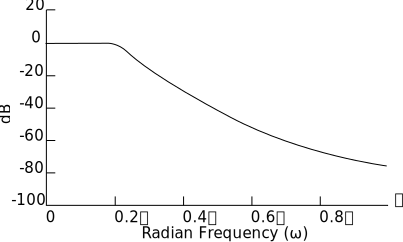
\includegraphics[width=1\textwidth]{imp_inv.pdf}
        \vspace{2mm}
        \caption{Frequency response using impulse invariance method\citep{oppenheim}.}
        \label{fig:impulse_invariance}
    \end{subfigure} 
    \hspace{4mm} 
\begin{subfigure}[b]{0.48\textwidth}
        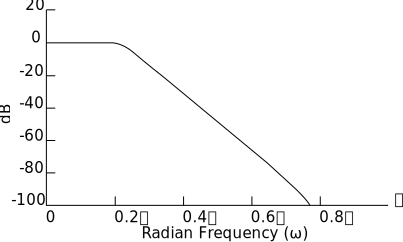
\includegraphics[width=1\textwidth]{bilin_transf.pdf}
        \vspace{2mm}
        \caption{Frequency response using bilinear transformation\citep{oppenheim}.}
        \label{fig:bilinear_transform}
    \end{subfigure}  
\caption{Comparison between the impulse invariance method and bilinear transformation.}
\label{fig:filter_design_methods}
\end{figure}

\begin{figure}[H]
    \centering
    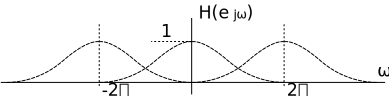
\includegraphics[width = 0.6\textwidth]{alias_imp.pdf}
    \caption{Aliasing when using the impulse invariance transform.}
    \label{fig:aliasing}
\end{figure} 
The second method for transforming from the s-plane to the z-plane is the bilinear transformation. The design approach is to design a continuous time filter and then map the imaginary $j\Omega$-axis of the s-plane into the unit circle of the z-plane \citep[p. 528]{oppenheim}. This means, that all frequencies in continuous time, $-\infty \le \Omega \le \infty$, are mapped into $-\pi \le \omega \le \pi$ in discrete time as shown in \autoref{fig:map_s2z}.
\begin{figure}[H]
    \centering
    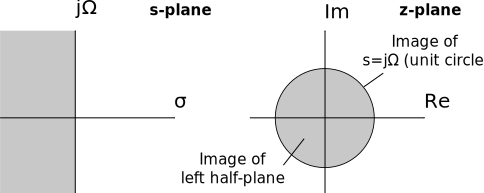
\includegraphics[width = 0.6\textwidth]{maping_s_to_z.pdf}
    \caption{Mapping the s-plane into z-plane\citep[p.528]{oppenheim}. The left side of the of s-plane is mapped within the unit circle of the z-plane, while the $j\Omega$-axis is mapped onto the unit circle.}
    \label{fig:map_s2z}
\end{figure} 
When bilinear transform is used, the relation between the frequency axis for the continuous time filter and the frequency axis for the discrete time filter, is no longer linear compared to the impulse invariance. This is shown in \autoref{fig:con2dis_freq}.
\begin{figure}[H]
    \centering
    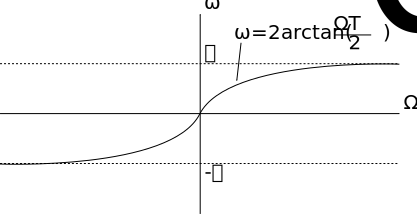
\includegraphics[width = 0.5\textwidth]{cont_to_dis.pdf}
    \caption{Frequency wrapping between continuous time and discrete time \citep[p.530]{oppenheim}.}
    \label{fig:con2dis_freq}
\end{figure} 
The relation between the frequency axis for the continuous time and discrete time filter is given as:
\begin{align}
\omega = 2\cdot \text{arctan}(\frac{\Omega T_s}{2}) \Leftrightarrow \Omega = \frac{2}{T_s}\tan (\frac{\omega}{2})
\label{bilinear_trans}
\end{align}
Comparing \autoref{bilinear_trans} to \autoref{impulse_inv2}, where the frequency axis $\omega$ has a linear scaling, the $\omega$-axis when using the bilinear transformation is not using a linear scaling. As a result, the frequency response of the digital filter is shown in \autoref{fig:bilinear_transform}. For the bilinear transformation there is no aliasing problem, and the filter keeps its characteristics. It has been chosen that the bilinear transformation will be used to transform from continuous time to discrete time.

\subsection{Designing Low-pass Filter for Encoders}
The digital filter for the encoders will now be designed. To determine the order, N, and the cutoff frequency, $\Omega_c$, of a Butterworth filter, the magnitude-squared function for a Butterworth filter is used\citep[p. 525]{oppenheim} to derive N and $\Omega_c$. 
\begin{align}
|H(j\Omega)|^2 = \frac{1}{1+(\frac{\Omega}{\Omega_c})^{2 \cdot N}}
\label{mag_sq}
\end{align}
\begin{where}
\va{$\Omega$}{is the frequency with the $|H(j\Omega)|$ attenuation}{rad/s}\\
\va{$\Omega_c$}{is the cutoff frequency}{rad/s}\\
\va{$N$}{is the order of the filter}{1}\\
\end{where}

By using the values from the specifications for the encoders and sensors the order and cutoff frequency can be solved. However since the filter is designed in continuous time, the frequencies specified from the specification needs to be transformed into continuous time. To do so, the frequency is warped from discrete time to continuous time using frequency warping \citep[p. 529]{oppenheim}, where the $s$ component is substituted with an expression for $z$. Frequency warping is given as:
\begin{align}
\Omega = \frac{2}{T_s} \cdot \tan(\frac{\omega}{2}) \Leftrightarrow \Omega = 2\cdot f_s \cdot \tan(\frac{\omega}{2})
\label{prewarp}
\end{align}
Frequency warping is now applied to the frequencies from the specification:
\begin{align}
\Omega_p &= 2 \cdot 1000 \cdot \tan(\frac{\frac{1}{100} \pi}{2}) = 31.418 \, \text{rad/s}\\
\Omega_s &= 2 \cdot 1000 \cdot \tan(\frac{\frac{3}{25} \pi}{2}) = 381.52 \, \text{rad/s}
\label{prewarp_calc}
\end{align}
\begin{where}
\va{$\Omega_p$}{is the passband frequency}{rad/s}\\
\va{$\Omega_s$}{is the stopband frequency}{rad/s}\\
\end{where}

The passband frequency and stopband frequency from \autoref{prewarp_calc} are inserted in equation \autoref{mag_sq} yielding:
\begin{align}
0.89125^2 = \frac{1}{1+(\frac{31.418 \text{rad/s}}{\Omega_c})^{2 \cdot N}}, \quad 0.0001^2 = \frac{1}{1+(\frac{381.52 \text{rad/s}}{\Omega_c})^{2 \cdot N}}
\label{mag_sq_calc}
\end{align}
The equations are solved with respect to $N$ and $\Omega_c$.
\begin{align}
N = 3.96 	\quad \text{and} \quad \Omega_c = 37.26 \, \text{rad/s}
\label{mag_sq_res}
\end{align}
The result yields that the minimum order of the filter is $N=4$ and the cutoff frequency is $\Omega_c = 37.26 \, \text{rad/s}$. It is important to state that since it is a 4th order filter, a phase shift of 180$\degree$ will occur at the cutoff frequency, which is undesirable. To minimize the phase shift at 37.26 rad/s, the cutoff frequency must be increased by one decade to $\Omega_c = 372.6 \, \text{rad/s}$. This trade-off ensures a low phase shift at 37.26 rad/s but lowers the amount of attenuation.

The next step is to determine the pole locations of the filter. The poles for a Butterworth filter can be found as \citep[p. 1041]{oppenheim}:
\begin{align}
p_k = \Omega_c \cdot e^{\frac{j\pi}{2N}\cdot (2k+N-1)}, \quad k=0,1, ..., 2N-1
\label{det_poles}
\end{align}
\begin{where}
\va{$p_k$}{is the pole location}{1}\\
\end{where}

When inserting the values of $k$ and $N$, the location of the poles can be found. However since a stable filter is desired, only the poles located in the left half plane of the s-plane are used. Since the order of the filter is $N=4$, $k$ is equal to 7. The pole locations are now found.
\begin{align}
p_1 &= \Omega_c \cdot e^{j \frac{5}{8} \pi}\\
p_2 &= \Omega_c \cdot e^{-j \frac{5}{8} \pi}\\
p_3 &= \Omega_c \cdot e^{j \frac{7}{8} \pi}\\
p_4 &= \Omega_c \cdot e^{-j \frac{7}{8} \pi}
\label{det_poles_res}
\end{align}
It is now possible to obtain the general transfer function of the continuous time filter from the pole locations. The general form of the transfer function for a Butterworth filter is given as:
\begin{align}
H_c(s) = \frac{G}{\prod\limits_{k=1}^{N}(s-p_k)} 
\label{trans_func_general}
\end{align}
\begin{where}
\va{$G$}{is the gain of the transfer function}{rad/s}\\
\va{$H_c(s)$}{is the continuous time transfer function}{rad/s}\\
\end{where}

Since the order of the filter is even, no poles are located on the real axis, and all poles have a pole pair because of the symmetric placement of the poles around the imaginary axis \citep[p. 1041]{oppenheim}. Due to the symmetry, it is possible to write $p_2$ as $p_1$ conjugated which is noted as $p_1^*$. This applies as well for $p_3$ and $p_4$.
\begin{align}
H_c(s) 	&= \frac{G}{(s-p_1) \cdot (s-p_1^*) \cdot (s-p_3) \cdot (s-p_3^*)} = \frac{G}{(s^2-p_1 s - p_1^*s - p_1 p_1^*) \cdot (s^2-p_3 s - p_3^* s - p_3 p_3^*)}
\label{trans_func_red}
\end{align}
The poles from \autoref{det_poles_res} are inserted in \autoref{trans_func_red}. 
\begin{align}
H_c(s) 	&= \frac{G}{(s^2-\Omega_c e^{j \frac{5}{8} \pi}s - \Omega_c e^{-j \frac{5}{8} \pi}s + \Omega_c^2 e^{j \frac{5}{8} \pi} e^{-j \frac{5}{8} \pi}) \cdot (s^2-\Omega_c e^{j \frac{7}{8} \pi}s - \Omega_c e^{-j \frac{7}{8} \pi}s + \Omega_c^2 e^{j \frac{7}{8} \pi} e^{-j \frac{7}{8} \pi})}
\label{trans_func_red_ins}
\end{align}
Because of the conjugated pole pairs, the mathematical rules $e^{j\omega}e^{-j\omega} = 1$ and $e^{j\omega}+e^{-j\omega} = \cos (\omega)$ are applied to \autoref{trans_func_red_ins}, which simplifies the transfer function.
\begin{align}
H_c(s) &= \frac{G}{(s^2 - 2\Omega_c \cos (\frac{5}{8} \pi)s + \Omega_c^2) \cdot (s^2 - 2\Omega_c \cos (\frac{7}{8} \pi)s + \Omega_c^2)}
\label{trans_func_red_ins2}
\end{align}
The final step is to determine the DC gain, $G$. The components are set to zero because a DC gain has a frequency of 0.
\begin{align}
|H_c(s)|\bigg|_{s=0} 	&= 1 =\frac{G}{\Omega_c^4}\\ 
G &= \Omega_c^4
\label{trans_func_red_ins3}
\end{align}
The transfer function of the filter in continuous time is now derived. The frequency response of the continuous time filter is now plottet:
\begin{figure}[H]
    \centering
    \includegraphics[width = 0.95\textwidth]{filters/continuous_bode_enc2.pdf}
    \caption{Frequency response of continuous time filter for the encoders.}
    \label{fig:continuous_bode_enc}
\end{figure}
As seen in \autoref{fig:continuous_bode_enc} the continuous time filter has the desired cutoff, pass band, and stop band frequency and complies with the minimum requirements. The continuous time filter will now be transformed into discrete time.

By using the bilinear transformation, the s-plane are mapped into the z-plane. The expression for the bilinear transformation is given as \citep[p. 528]{oppenheim}:
\begin{align}
s = \frac{2}{T_s}\cdot \frac{z-1}{z+1}
\label{bilinear_trans2}
\end{align}
Applying the bilinear transformation on the transfer function yields:
\begin{align}
H_{enc}(z) &= \frac{\Omega_c^4}{((\frac{2}{T_d}\frac{z-1}{z+1})^2 - 2\Omega_c \cos (\frac{5}{8} \pi)\frac{2}{T_d}\frac{z-1}{z+1} + \Omega_c^2) \cdot ((\frac{2}{T_d}\frac{z-1}{z+1})^2 - 2\Omega_c \cos (\frac{7}{8} \pi)\frac{2}{T_d}\frac{z-1}{z+1} + \Omega_c^2)}
\label{trans_func_disc_ins}
\end{align}
\begin{where}
\va{$H_{enc}(z)$}{is the discrete time transfer function of the digital filter for the encoders}{Hz}\\
\end{where}

The values for the variables are inserted and the expression of $H_d(z)$ is afterwards reduced to a standard form where the first denominator coefficient, $a_0$ is equal to 1 \citep[p. 456]{oppenheim}. The form is more efficient in the matter of implementation, which will be discussed later.
\begin{align}
H_{enc}(z) = \frac{\sum\limits_{k=0}^{M}(b_kz^{-k})}{1 - \sum\limits_{k=1}^{N}(a_kz^{-k})} 
\label{trans_standard}
\end{align}
Reducing the expression from \autoref{trans_func_disc_ins} to the form in \autoref{trans_standard}, the transfer function for the digital low-pass Butterworth filter is:

\begin{align}
H_{enc}(z) = \frac{0.000742+0.002969z^{-1}+0.00445z^{-2}+0.002969z^{-3}+0.000742z^{-4}}{1-3.039809z^{-1}+3.554178z^{-2}-1.881894z^{-3}+0.379401z^{-4}}
\label{transfer_func_enc}
\end{align}

The magnitude of the frequency response is now plotted to examine if the frequency response has the desired characteristic.

\begin{figure}[H]
    \centering
    \includegraphics[width = 0.8\textwidth]{filters/frequency_response_encoder2.pdf}
    \caption{Frequency response of the 4th order low-pass discrete digital filter for the encoders. The black line is the frequency response and the blue line is the phase response.}
    \label{fig:freq_response_enc}
\end{figure} 
As shown in \autoref{fig:freq_response_enc} the magnitude frequency response has the desired characteristics with 3 dB attenuation at 58.6 Hz and only -12.64$\degree$ phase shift at 5 Hz compared to 180$\degree$ phase shift at the cutoff frequency.

\subsection{Low-pass Filter for Sensors}
Designing the low-pass Butterworth filter for the sensors is similar to the filter for the encoders. However instead of determining the cutoff frequency and order, they are set to 15 Hz and 3rd order as stated in the requirement and specification section. After applying frequency warping the cutoff frequency is increasing by one decade to minimize the phase shift at 15 Hz. The cutoff frequency is determined to be $\Omega_c = 1138.7 \, \text{rad/s}$. Since the order is known, the poles of the 3rd order low-pass filter is determined by \autoref{det_poles}.
\begin{align}
p_1 &= \Omega_c \cdot e^{j \frac{2}{3} \pi}\\
p_2 &= \Omega_c \cdot e^{-j \frac{2}{3} \pi}\\
p_3 &= \Omega_c \cdot e^{j\pi} = -\Omega_c 
\label{det_poles_res2}
\end{align}
The poles are now inserted in \autoref{trans_func_general}. Since one of the poles is on the real axis, the pole does not have a complex conjugated pole pair around the real axis. 
\begin{align}
H_c(s) &= \frac{G}{(s + \Omega_c) \cdot (s^2 - 2\Omega_c \cos (\frac{2}{3} \pi)s + \Omega_c^2)}
\label{trans_func_red_ins22}
\end{align}
The DC gain is determined by setting $s$ to zero. The gain is then derived to be $\Omega_c^3$. 
\begin{figure}[H]
    \centering
    \includegraphics[width = 0.85\textwidth]{filters/continuous_bode_gyro2.pdf}
    \caption{Frequency response of continuous time filter for the sensors.}
    \label{fig:continuous_bode_gyro}
\end{figure}
The filter has the desired cutoff frequency, since the calculated frequency warped cutoff frequency was determined to $\Omega_c = 1138.7 \, \text{Hz}$. To transform the continuous time filter into discrete, the bilinear transform is used with the inserted cutoff frequency. Afterwards the expression is reduced to the standard form seen in \autoref{trans_standard}.
\begin{align}
H_{sen}(z) = \frac{0.790712+2.37213z^{-1}+2.37213^{-2}+0.790712z^{-3}}{1+2.53247z^{-1}+2.16800z^{-2}+0.625224z^{-3}}
\label{transfer_func_gyro}
\end{align}
\begin{where}
\va{$H_{sen}(z)$}{is the discrete time transfer function of the digital filter for the encoders}{Hz}\\
\end{where}

Plotting the frequency response of the transfer function, reveals that the cutoff frequency is located at 31 Hz with a phase shift on 135$\degree$. The phase shift at 15 Hz is 11.46$\degree$.

\begin{figure}[H]
    \centering
    \includegraphics[width = 0.9\textwidth]{filters/frequency_response_gyro2.pdf}
    \caption{Frequency response of the 3rd order low-pass digital filter for the sensors. The black line is the frequency response and the blue line is the phase response.}
    \label{fig:freq_response_sensor}
\end{figure} 
In the next section an analysis of how to implement the derived transfer functions of the digital filters in a microcontroller follows.
\section{Implementation of Digital Filters}
The derived transfer functions for filters need to be implemented in a microcontroller. Since the microcontroller only works in time domain where the input of the system is $x[n]$ and output $y[n]$, the filters need to be transformed back to discrete time domain from the z-domain. The primary purpose of this section is to analyse how to do the inverse z-transformation and implement the filters efficiently.

In discrete time domain, the output of a system is given as the convolution of the input with the system impulse response:
\begin{align}
y[n] = \sum\limits_{k=-\infty}^{\infty}x[k] h[n-k] = x[n]*h[n]
\label{time_domain_output}
\end{align}
When applying the z-transform in \autoref{time_domain_output}, the convolution is substituted with a multiplication in the z-domain.
\begin{align}
y[n] = x[n]*h[n] \xleftrightarrow{Z} Y(z) = H(z) X(z)
\label{z_domain}
\end{align}
\begin{where}
\va{$y[n]$}{is the discrete time output}{1}\\
\va{$x[n]$}{is the discrete time input}{1}\\
\va{$h[n]$}{is the discrete time impulse response}{1}\\
\end{where}

The expression of $H(z)$ is previously found to be the discrete time transfer function of the digital filter which is written as:
\begin{align}
H(z) = \frac{Y(z)}{X(z)} =\frac{\sum\limits_{k=0}^{M}(b_kz^{-k})}{\sum\limits_{k=0}^{N}(a_kz^{-k})} \Rightarrow \sum\limits_{k=0}^{N}(a_kz^{-k})Y(z) = \sum\limits_{k=0}^{M}(b_kz^{-k})X(z)
\label{z_domain_trans}
\end{align}
Since the coefficient, $a_0$, for both derived transfer functions are $a_0 = 1$, because \autoref{trans_standard} are used to derive the transfer functions, the following difference equation may be written.
\begin{align}
Y(z) = -\sum\limits_{k=1}^{N}(a_kz^{-k})Y(z) + \sum\limits_{k=0}^{M}(b_kz^{-k})X(z)
\label{z_domain_trans2}
\end{align}
Because of the coefficient $a_0 = 1$, the equation may be written as \autoref{z_domain_trans2}, where $k=1$ for the first summation of $a_k$. If $a_0 \not= 1$ the difference equation should be divided by $a_0$ on both sides of the equation.

One of the properties of transforming between discrete time domain and the z-domain is the time-shifting property \citep[p. 131]{oppenheim}. The time-shifting property is basically that a factor of $z^{-k}$ will correspond to a delayed sample in discrete time domain.
\begin{align}
x[n-k] \xleftrightarrow{Z} z^{-k} X(z)
\label{time_shifting}
\end{align}

\autoref{time_shifting} also applies for $Y(z)$. The inverse z-transform from \autoref{z_domain} are therefore now applied in \autoref{z_domain_trans2} with the time-shifting property from \autoref{time_shifting}. This yields the following difference equation of the output $y[n]$.
\begin{align}
y[n] = -\sum\limits_{k=1}^{N}a_ky[n-k] + \sum\limits_{k=0}^{M}b_kx[n-k]
\label{time_domain2}
\end{align}
To determine the output of the filters, \autoref{z_domain_trans} is first applied to the transfer function of the filter. Afterwards the expression is rewritten to the difference equation in \autoref{z_domain_trans2}. Lastly the inverse z-transformation is used to transform the equation from z-domain to time domain with the end result seen in \autoref{time_domain2}.

When using the procedure above, for the transfer functions for the digital filters,  the following difference equations are derived. For the encoders:
\begin{align}
\begin{split}
y_{enc}[n] 	=& -(a_1y[n-1] + a_2y[n-2] + a_3y[n-3] + a_4y[n-4]) + b_0x[n] + b_1x[n-1]\\
			&  + b_2x[n-2] + b_3x[n-3] + b_4x[n-4] \\
			&\Downarrow \\
y_{enc}[n] 	=& -(-3.039809y[n-1] + 3.554178y[n-2] + (-1.881894)y[n-3]  \\ 
			&  + 0.079401y[n-4]) + 0.000742x[n] + 0.002969x[n-1] \\
			&  + 0.004453x[n-2] + 0.002969x[n-3] + 0.000742x[n-4]
\end{split}
\label{enc_diff}
\end{align}
\begin{where}
\va{$y_{enc}[n]$}{is the discrete time output of the digital filters for the encoders}{1}\\
\end{where}
The same procedure is applied for the digital filter for the sensors.
\begin{align}
\begin{split}
y_{sen}[n] 	=& -(a_1y[n-1] + a_2y[n-2] + a_3y[n-3]) + b_0x[n] + b_1x[n-1]\\
			&  + b_2x[n-2] + b_3x[n-3] \\
			&\Downarrow \\
y_{sen}[n] 	=& -(2.53247y[n-1] + 2.16800y[n-2] + 0.625224y[n-3])  \\ 
			&  + 0.790712x[n] + 2.37213x[n-1] + 2.37213x[n-2] + 0.790712x[n-3] \\
\end{split}
\label{sen_diff}
\end{align}
\begin{where}
\va{$y_{sen}[n]$}{is the discrete time output of the digital filters for the sensors}{1}\\
\end{where}

As the difference equation of the output $y[n]$ for both the encoders and sensors are derived, the next step is to realize the equations in the microcontroller.
\subsection{Filter Structure Optimization and Code Implementation}
There are different ways to implement the difference equation of the output $y[n]$ derived from the previous section. This section primarily discusses different filter structures to implement in the microcontroller. It is possible to implement \autoref{enc_diff} and \autoref{sen_diff} directly to the microcontroller. However doing so is not necessarily computational efficient for the microcontroller compared to other alternatives. The IIR filter structures are illustrated as block diagrams which eases the readability.
\begin{figure}[H]
    \centering
    \includegraphics[width = 0.8\textwidth]{filter_implementation_gyro_simulink_illustration.pdf}
    \caption{Filter structure of the IIR 3rd order digital filter for the sensors. There is a feedback loop at the output, which can make the filter unstable if not designed carefully.}
    \label{fig:filter_implementation_gyro_simulink_illustration}
\end{figure} 
If the difference equation from \autoref{sen_diff} is implemented directly in the microcontroller, the filter structure of the equation is shown in \autoref{fig:filter_implementation_gyro_simulink_illustration}. The type of structure is called direct form I \citep[p. 399]{oppenheim} and implementing such a structure requires six variables to store the values of $x[n-1]$, $x[n-2]$, $x[n-3]$, $y[n-1]$, $y[n-2]$ and $y[n-3]$. An alternative way of implementing the filter is using direct form II. The output of this structure is equivalent to direct form I, but needs only four variables to store values. The filter for direct form II is seen in \autoref{fig:filter_implementation_gyro_simulink}.
\begin{figure}[H]
    \centering
    \includegraphics[width = 0.65\textwidth]{filter_implementation_gyro_simulink.pdf}
    \caption{Filter structure of the 3rd order IIR filter for the sensors. Direct form II.}
    \label{fig:filter_implementation_gyro_simulink}
\end{figure} 
The direct form II is used for the digital filter for the sensors. For the direct form II, variables are inserted before and after every delay ending with a total number of variables of four. This saves memory and the processor spares at least two additional instructions for copying the value in a variable to another, corresponding to a delay. The code implementation of the filter structure is seen in \autoref{lst:enc_code}. 

\lstset{language=C, caption={Code implementation of 3th order low pass filter for the sensors. Direct form II.}, label=lst:sensor_code}
\begin{lstlisting}
double IIR_LP_ANG(double angle){
	static double BUF0, BUF1, BUF2, BUF3 = 0;	// Initialize the buffers of static doubles
	static double angleFiltered = 0;			// Initialize the output variable
	
	BUF0 = angle - (a1*BUF1 + a2*BUF2 + a3*BUF3); // Calculate the first buffer
	angleFiltered = b0*BUF0 + b1*BUF1 + b2*BUF2 + b3*BUF3; // Calculate the output
	BUF3 = BUF2; // Shift the buffer by 1 sample. Corresponds to a delay.
	BUF2 = BUF1;
	BUF1 = BUF0;
	
	return angleFiltered;
}
\end{lstlisting}
The variables are initialized as static doubles, since values can be large and the values need to be preserved when the function is returned. The "static" for the angleFiltered is however done to prevent allocating memory every time the function is called. In the next two lines calculations for the filter are processed. The algorithm is derived from the filter structure in \autoref{fig:filter_implementation_gyro_simulink}. Afterwards the values in the variables are shifted, which correspond to a delayed sample.

The filter for the encoders needs to be implemented as well. However instead of implementing the filter using direct form II with four delays, the structure is rearranged into biquad cascade form, which consists of two 2nd order low-pass filters in direct form II. The filter structure of the filter is seen in \autoref{fig:filter_implementation_encoder_simulink_illustration}.

\begin{figure}[H]
    \centering
    \includegraphics[width = 0.9\textwidth]{filter_implementation_encoder_simulink_illustration.pdf}
    \caption{Filter structure of the 4th order IIR filter for the encoders.}
    \label{fig:filter_implementation_encoder_simulink_illustration}
\end{figure} 
Rearranging the filter structure from direct form I to biquad cascade direct form II requires that the transfer function is rewritten into the following form\citep[p. 409]{oppenheim}:
\begin{align}
H_d(z) = \prod\limits_{k=1}^{N_s}\frac{b_{0k}+b_{1k}z^{-1}+b_{2k}z^{-2}}{1+a_{1k}z^{-1}+a_{2k}z^{-2}}
\label{cascade_form}
\end{align}
Since the order of the filter is 4, $N_s = 2$. Using \autoref{cascade_form} the transfer function may be split into two 2nd order transfer functions.
\begin{align}
\begin{split}
H_{enc}(z) 	&= H_{enc1}(z)H_{enc2}(z) \\
		&\Downarrow \\
H_{enc}(z) 	&= \frac{0.027244+0.054488z^{-1}+0.027244z^{-2}}{1-1.400000z^{-1}+0.50069z^{-2}} \cdot \frac{0.027244+0.054488z^{-1} + 0.027244z^{-2}}{1 - 1.639811z^{-1} + 0.757754z^{-2}}
\end{split}
\label{cascade_transfer}
\end{align}
\begin{where}
\va{$H_{enc1}(z)$}{is the 2nd order transfer function of the first biquad}{1}\\
\va{$H_{enc2}(z)$}{is the 2nd order transfer function of the second biquad}{1}\\
\end{where}

With the transfer function from \autoref{cascade_transfer} the $a_k$ and $b_k$ coefficients are now derived. The procedure for implementing the filter is to use the coefficients and design the algorithm from the filter structure in \autoref{fig:filter_implementation_encoder_simulink_illustration}. The implemented code is shown in \autoref{lst:enc_code}.\newpage

\lstset{language=C, caption={Code implementation of 4th order low pass filter for the encoders.}, label=lst:enc_code}
\begin{lstlisting}
double IIR_LP_ENC(double vel){
	static double BUF01, BUF11, BUF21 = 0; // Initialize buffers for first biquad
	static double BUF02, BUF12, BUF22 = 0; // Initialize buffers for second biquad
	static double W, vel_filt = 0;		// W is the output for the first biquad
								
	BUF01 = vel - (a11*BUF11 + a21*BUF21); // Algorithm for first biquad
	W = b01*BUF01 + b11*BUF11 + b21*BUF21;
	BUF21 = BUF11;						// Shift values in buffers
	BUF11 = BUF01;

	BUF02 = W - (a12*BUF12 + a22*BUF22); // Algorithm for second biquad
	vel_filt = b02*BUF02 + b12*BUF12 + b22*BUF22;
	BUF22 = BUF12;
	BUF12 = BUF02;
	
	return vel_filt;
}
\end{lstlisting}

As shown in \autoref{lst:enc_code} the implementation of the cascade form is to process two 2nd order filters in direct form II, where the output of the first filter, $W$, is the input of the next filter.

\section{Results of Digital Filters}
The Butterworth filters are now designed and can be implemented in the microcontroller. Before implementing the code in the microcontroller, the algorithm for the filters are applied for the measurements to see their impact on the measurements. In \autoref{fig:filter_implementation_encoder} the comparison between the unfiltered and filtered signal from the encoder is shown. The digital filter attenuates measurements, which appears to be noise, greatly. The spectrogram in \autoref{fig:encoder_comp_spectrum} also shows the spectrum of the filtered signal. When comparing the spectrogram in \autoref{fig:encoder_comp_spectrum} and \autoref{fig:spectrogram_encoder}, it is seen that the filter attenuates signals above the cutoff frequency.  

\begin{figure}[H]
\centering
\begin{subfigure}[b]{0.85\textwidth}
\hspace*{-0.8cm} 
    \includegraphics[width = 1\textwidth]{filters/encoder_comp.pdf}
    \caption{Comparison between the original and the filtered encoder measurements. The noise is reduced greatly in the filtered version.}
    \label{fig:filter_implementation_encoder}
\end{subfigure}    
\begin{subfigure}[b]{0.9\textwidth}
    \includegraphics[width = 0.98\textwidth]{filters/encoder_comp_spectrum.png}
    \caption{Spectrogram of the filtered signal. Almost all frequencies above 300 Hz are filtered away.}
    \label{fig:encoder_comp_spectrum}
\end{subfigure}   
\caption{Comparison of the unfiltered and filtered signal and spectrogram of the filtered signal.}
\end{figure}

A test shows that the segway is still able to stabilise itself in an upright position, after applying the filters on the segway. The digital filters for the encoders are therefore working as expected.

The digital filter for the angle sensors need to be applied on some measurements as well. The comparison of the unfiltered and filtered signal for the sensors are shown in \autoref{fig:filter_implementation}. 

\begin{figure}[H]
    \centering
    \includegraphics[width = 0.93\textwidth]{filters/gyro_comp.pdf}
    \caption{Comparison between the original and the filtered angle measurements.}
    \label{fig:filter_implementation}
\end{figure}
As shown in \autoref{fig:filter_implementation} the implemented digital filter does not improve the measurements very much. Therefore it is chosen to not implement the digital filter for the angle.

If the filters are implemented, they do not allow the wireless communication to be executed. Since the wireless communication is of higher priority in the project, the digital filters will not be implemented as they take up too much computation time. The design and implementation of the remote controller for the segway follows in the next chapter.